%Created with command:
%"/home/josh/Teaching/trunk/Utilities/makeexam" "Homework 7 - Flip-flops and State Machines" "Please complete the problems below.  As usual you may work together.  However make sure the work that you submit is yours." "../LatchesAndFlipFlops/Assessments/wakerly_7_7.tex" "../StateMachines/Assessments/wakerly_7_18.tex" "../StateMachines/Assessments/wakerly_7_44.tex"
\documentclass{article}
\usepackage[T1]{fontenc}
\usepackage{arev}
\usepackage{longtable}
\usepackage[hmargin=2cm,vmargin=2cm]{geometry}
\usepackage{graphicx}
\usepackage{listings}
\setlength{\parindent}{0pt}
\title{Homework 7 - Flip-flops and State Machines}
\date{}
\begin{document}
\maketitle
Please complete the problems below.  As usual you may work together.  However make sure the work that you submit is yours. (24 points total)
\begin{longtable}[l]{rp{17cm}}
%file: ../LatchesAndFlipFlops/Assessments/wakerly_7_7.tex
1.&\begin{minipage}[t]{\linewidth}(4 pt) Do problem 7.7 in the text.  Your answer should be a logic diagram that includes any combinational gates and one or more T flip-flops to implement the J-K flip-flop. \\ \\

Solution: \\ \\
\begin{center}
  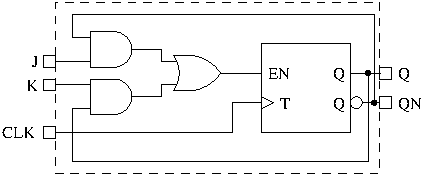
\includegraphics{../LatchesAndFlipFlops/Assessments/JKFlipFlop}
\end{center}
\end{minipage}\\
\medskip
%file: ../StateMachines/Assessments/wakerly_7_18.tex
2.&\begin{minipage}[t]{\linewidth}(10 pt) Do problem 7.18 in the text.  Please explicitly show each of the seven steps in the procedure for state machine analysis that we discussed in class. \\ \\

Solution: \\ \\
Step 1: Write the logic equations for the combinational input.
$$D2 = (D2 + D1)' \oplus (D1 \oplus D2)$$
$$D1 = D2$$
$$D0 = D1$$
Step 2: Write the transition equations. \\ \\
Characteristic equations for each flip-flop:
$$Q2* = D2$$
$$Q1* = D1$$
$$Q0* = D0$$
Transition equations:
$$Q2* = (D2 + D1)' \oplus (D1 \oplus D2)$$
$$Q1* = D2$$
$$Q0* = D1$$
Step 3: Construct the state table. \\ \\
\begin{tabular}{ccc|ccc}
  \textbf{Q2} & \textbf{Q1} & \textbf{Q0} & \textbf{Q2*} & \textbf{Q1*} & \textbf{Q0*} \\
  \hline
  0 & 0 & 0 & 1 & 0 & 0 \\
  0 & 0 & 1 & 0 & 0 & 0 \\
  0 & 1 & 0 & 1 & 0 & 1 \\
  0 & 1 & 1 & 0 & 0 & 1 \\
  1 & 0 & 0 & 0 & 1 & 0 \\
  1 & 0 & 1 & 1 & 1 & 0 \\
  1 & 1 & 0 & 1 & 1 & 1 \\
  1 & 1 & 1 & 0 & 1 & 1 \\
\end{tabular} \\ \\
Step 4: Assign state names and construct a state table. \\ \\
\begin{tabular}{c|c}
  \textbf{S} & \textbf{S*} \\
  \hline
  0 & 4 \\
  1 & 0 \\
  2 & 5 \\
  3 & 1 \\
  4 & 2 \\
  5 & 6 \\
  6 & 7 \\
  7 & 3 \\
\end{tabular} \\ \\
Step 5: Determine the output equations. \\ \\
$$Q2 = Q2$$
$$Q1 = Q1$$
$$Q0 = Q0$$
\end{minipage}\\
\newpage
&\begin{minipage}[t]{\linewidth}
Step 6: Construct the state/output table. \\ \\
\begin{tabular}{c|cc}
  \textbf{S} & \textbf{S*} & \textbf{Q2 Q1 Q0} \\ 
  \hline
  0 & 4 & 100 \\
  1 & 0 & 000 \\
  2 & 5 & 101 \\
  3 & 1 & 001 \\
  4 & 2 & 010 \\
  5 & 6 & 110 \\
  6 & 7 & 111 \\
  7 & 3 & 011 \\
\end{tabular} \\ \\
Step 7: Draw the state diagram. \\ \\
\begin{center}
  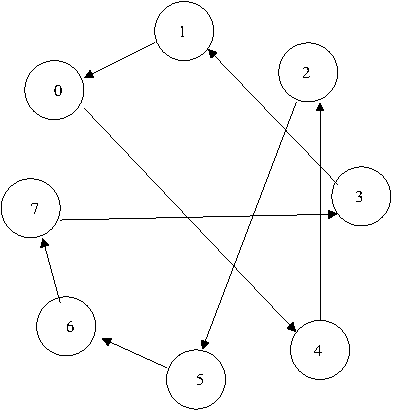
\includegraphics{../StateMachines/Assessments/Wakerly_7_18_StateDiagram}
\end{center}
\end{minipage}\\
\medskip
%file: ../StateMachines/Assessments/wakerly_7_44.tex
3.&\begin{minipage}[t]{\linewidth}(10 pt) Do problem 7.44 in the text. \\ \\

Solution: \\ \\
\begin{center}
  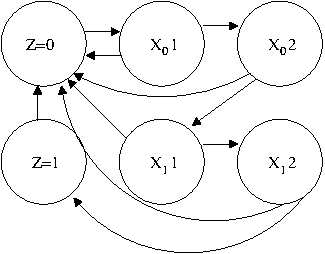
\includegraphics{../StateMachines/Assessments/Wakerly_7_44_StateDiagram}
\end{center}
\end{minipage}\\
\medskip
\end{longtable}
\end{document}
